\begin{figure}[H] \centering
\subsection{BDD (SK)}
{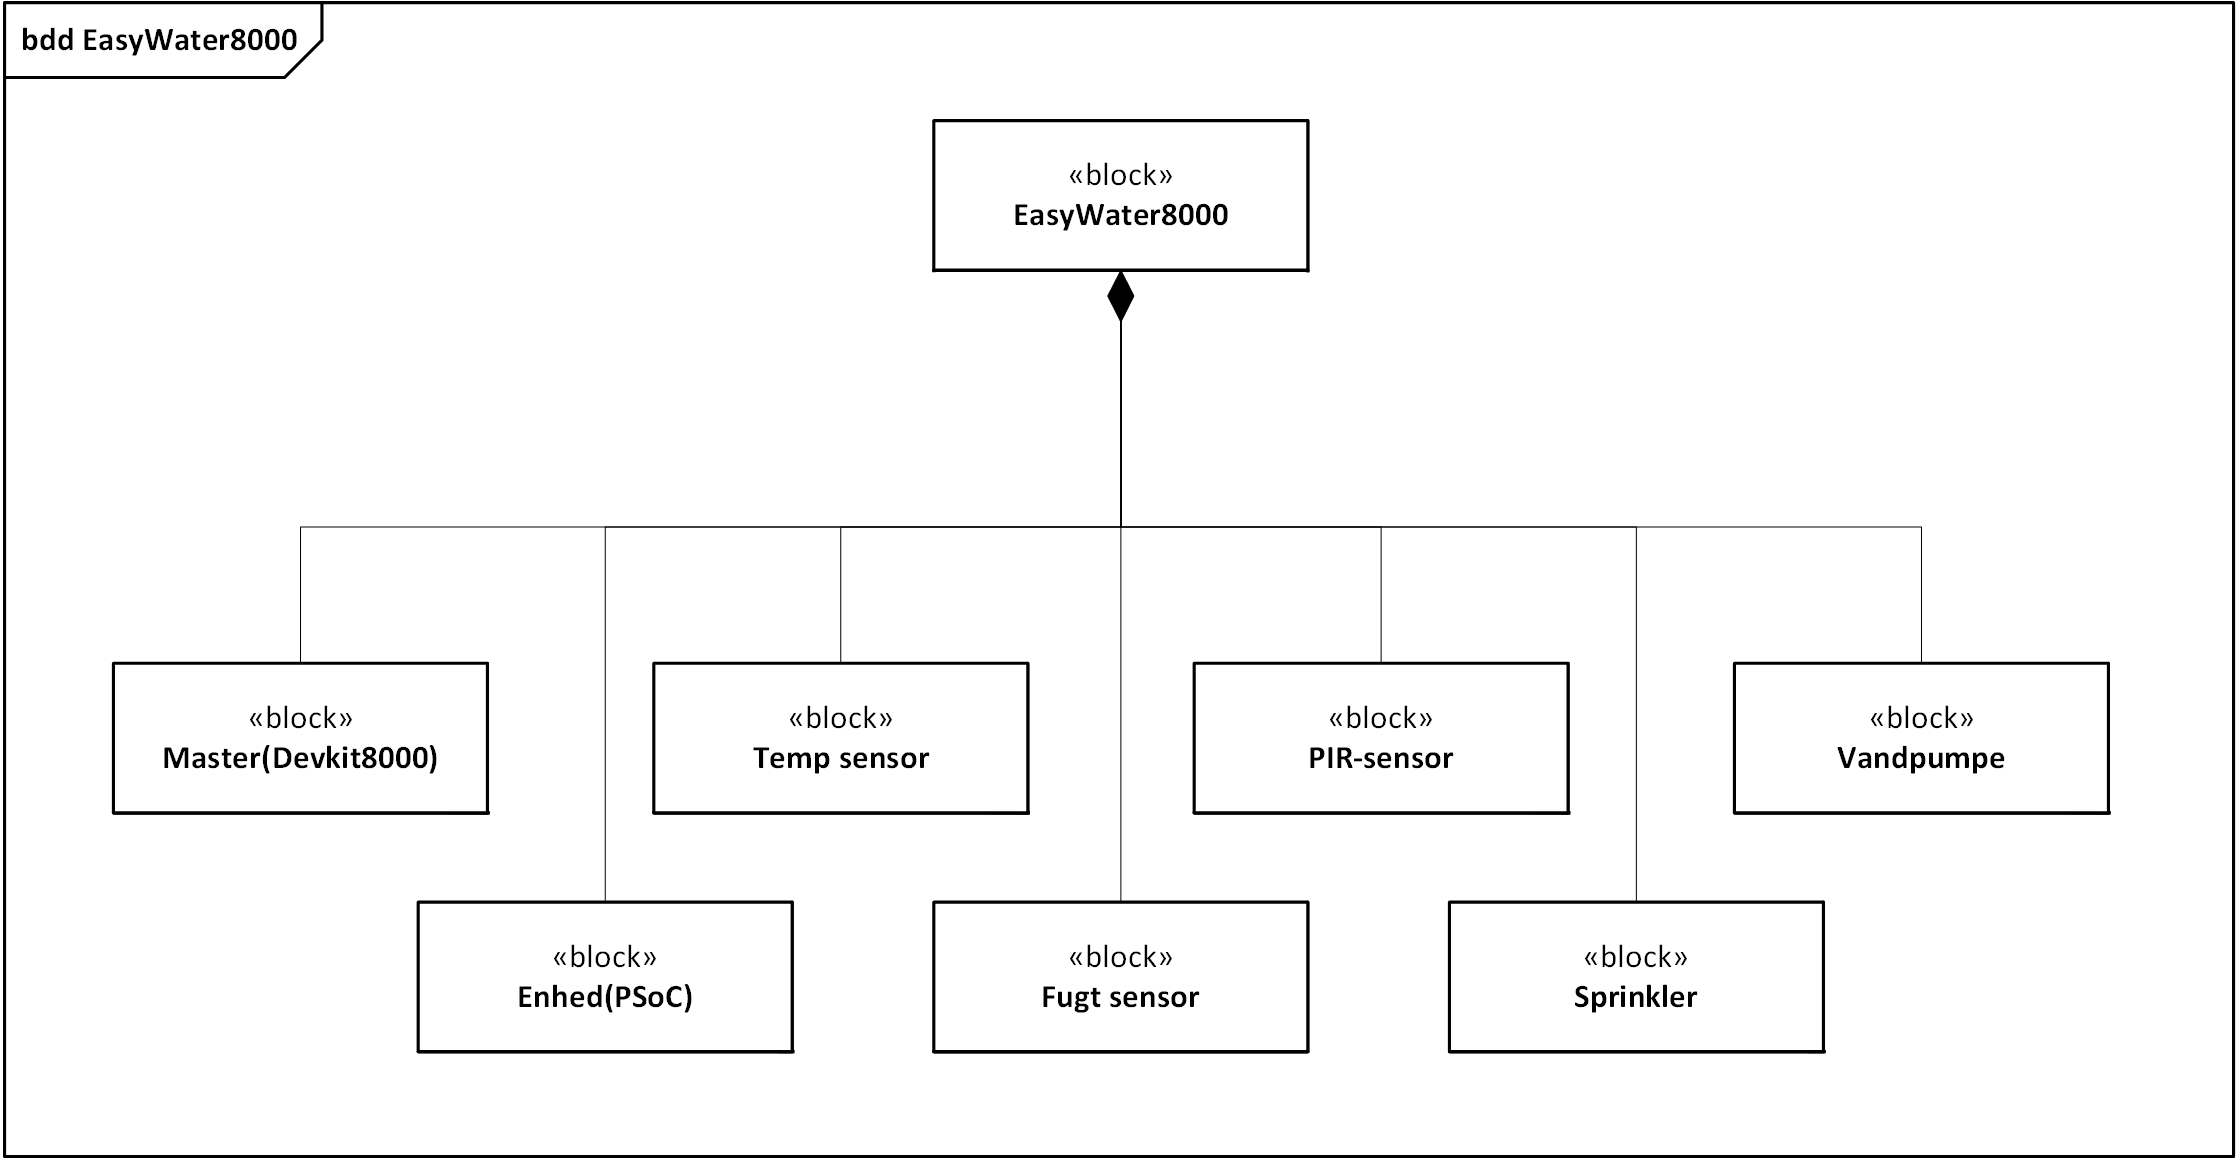
\includegraphics[width=0.9\textwidth]{filer/systemarkitektur/BDD}}
\caption{BDD}
\label{lab:bdd}
\raggedright
\end{figure}
BDD diagrammet giver et overblik over hvad det samlede EasyWater8000 system består af, samt indbyrdes multiplicitet. FT sensoren er en kombineret fugt- og temperatursensor.  \newline \newline

\begin{figure}[H] \centering
\subsection{BDD Master (MK)}
{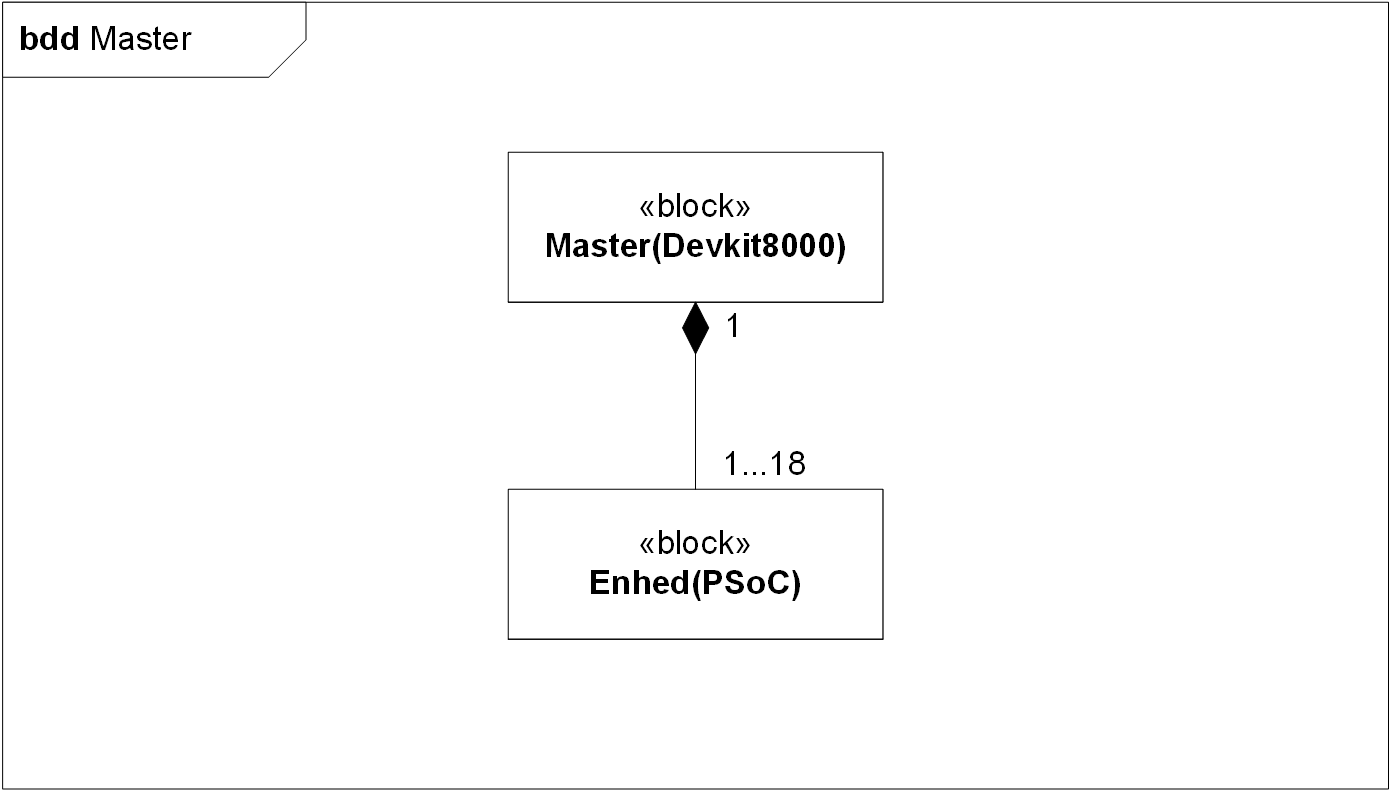
\includegraphics[width=0.7\textwidth]{filer/systemarkitektur/BDD_Master}}
\caption{BDD Master}
\label{lab:bddmaster}
\raggedright
\end{figure}
BDD diagrammet for Master, viser at Master består af ét Devkit8000, som kobles op med en til 18 Enheder.

\begin{figure}[H] \centering
\subsection{BDD Enhed (MK)}
{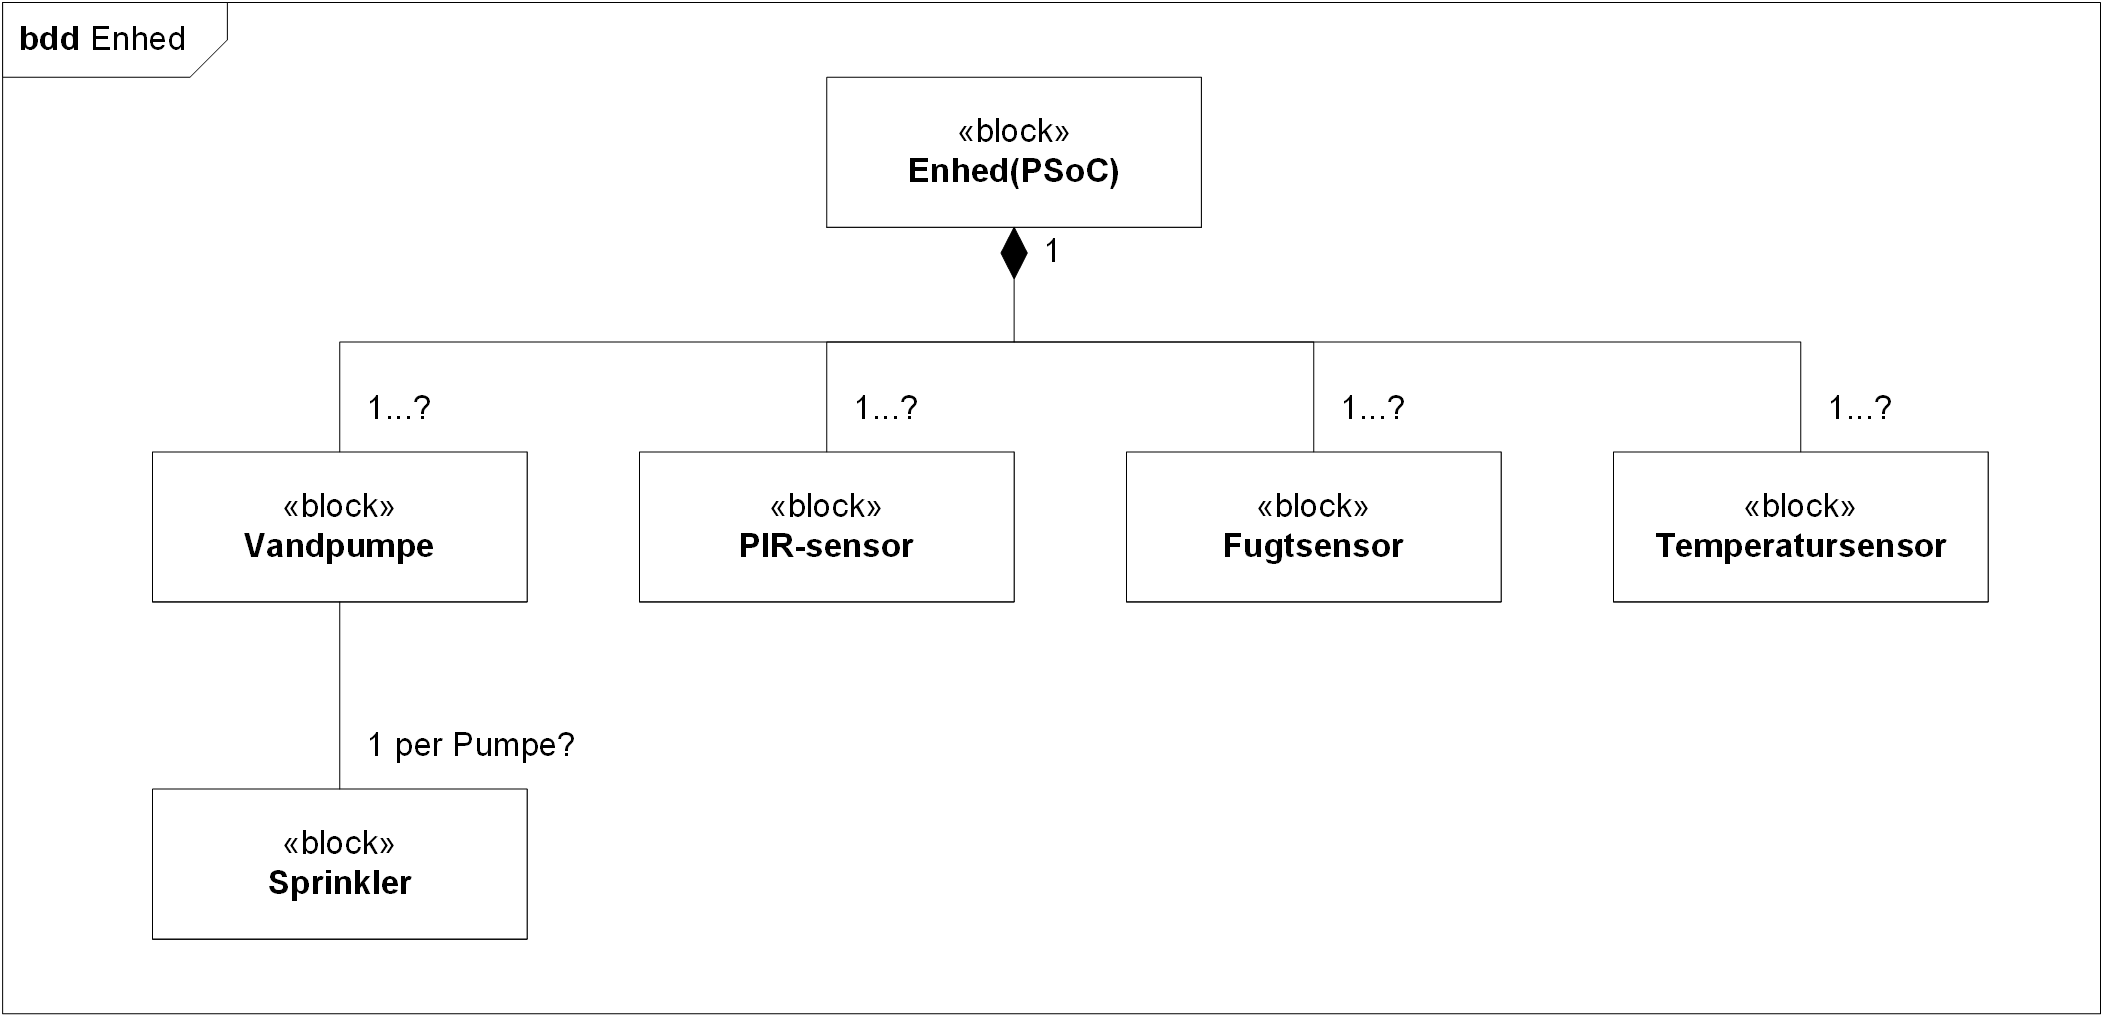
\includegraphics[width=0.9\textwidth]{filer/systemarkitektur/BDD_Enhed}}
\caption{BDD Enhed}
\label{lab:bddenhed}
\raggedright
\end{figure}
BDD diagrammet for Enhed, viser at én Enhed består af én PSoC som kan kobles sammen med op til 20 Vandpumper, 20 FT sensorer (Fugt- og Temperatursensorer) samt 1 PIR-sensor. Sprinkler bliver i systemet koblet sammen med én Vandpumpe.

\begin{figure}[H] \centering
\subsection{IBD (SK)}
{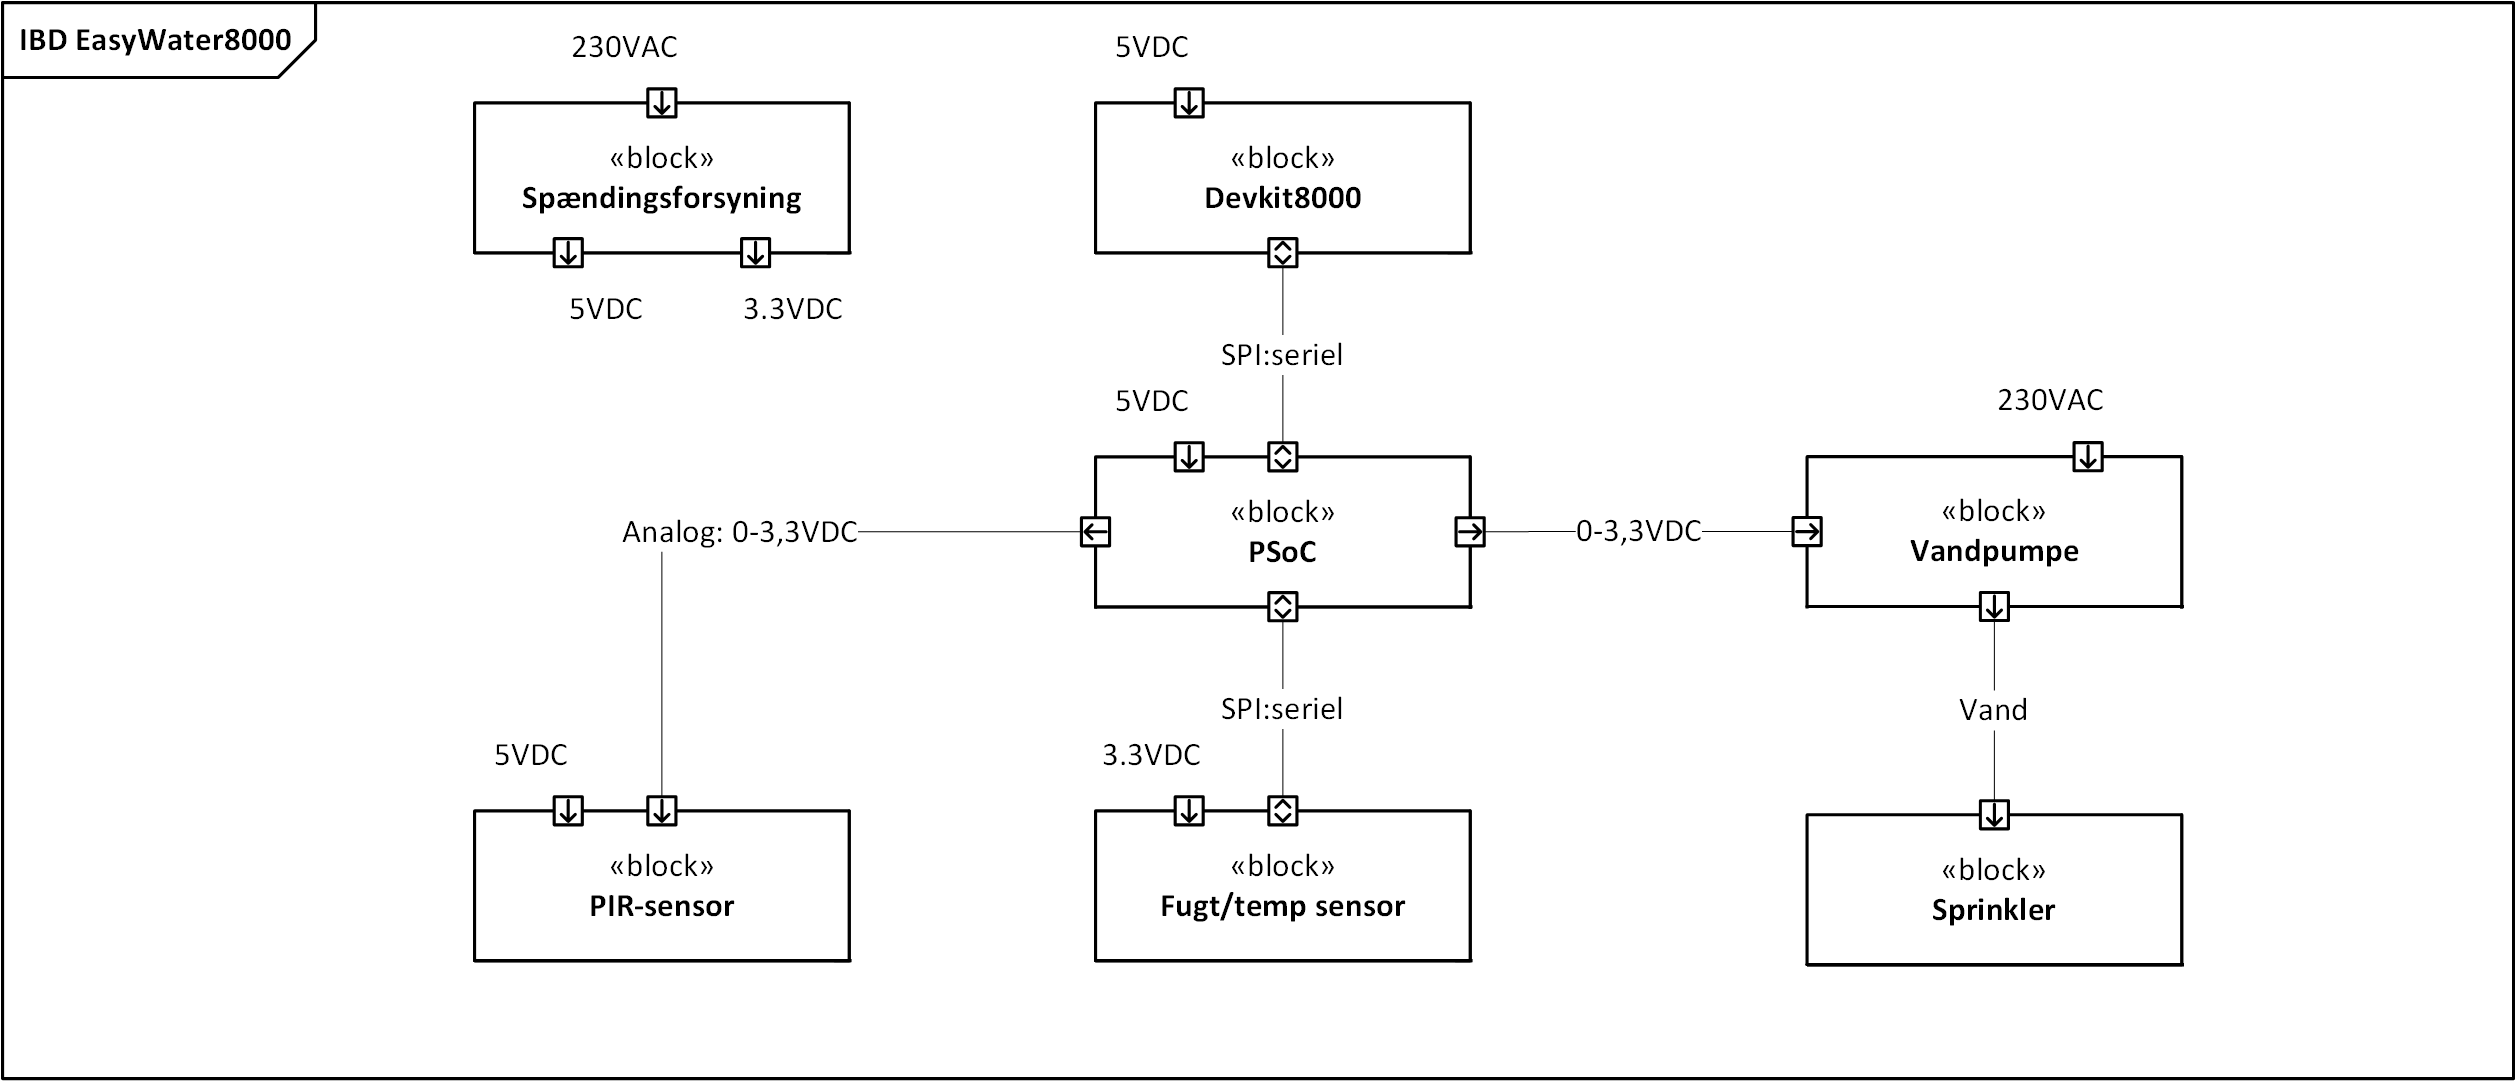
\includegraphics[width=0.9\textwidth]{filer/systemarkitektur/IBD}}
\caption{IBD}
\label{lab:ibd}
\raggedright
\end{figure}
IBD diagrammet giver et internt overblik over hvordan hele systemet er forbundet. Der ses hvilke typer signaler der bliver sendt imellem de forskellige blokke. \newline \newline
\textbf{Spændingsforsyning}: Spændingsforsyningens forbindelser er ikke påtegnet da dette ville give et uoverskueligt diagram, de er i stedet beskrevet med standardflowports. Spændingsforsyningen forsyner enhed (PSoC), FT sensor, PIR-sensor samt relæet i vandpumpen. Master(devkit8000) har sin egen spændingsforsyning.  \newline \newline
\textbf{FT sensor}: Blokken beskriver at fugt- og temperatursensor er integreret i en chip. \newline \newline
\textbf{Relæ styring}: Blokken beskriver at vandpumpen består af et relæ, der står for at tænde/slukke for den. \newline \newline

\begin{table}[H] %% Blok og Signal Tabel
\subsection{Grænseflade (HW)}
For at opnå forståelse for signalerne mellem blokkene laves en grænseflade beskrivelse, der beskriver de enkelte blokkes porte og hvilke signaler der løber imellem disse.

\subsubsection{Blok beskrivelse (HW)}
Til at beskrive blokkene nærmere anvendes tabeller som ses herunder. Her er hvert signal i en respektiv blok kommenteret og blokkens funktion er kort beskrevet. 

\caption{Tabel med beskrivelse af respektive blokke}
\begin{small}
\begin{tabular}{|p{3,3cm}|p{3,3cm}|p{3,3cm}|p{3,3cm}|}
\hline
\textbf{Bloknavn} & \textbf{Funktion} & \textbf{Signaler} & \textbf{Kommentar} \\ \hline

Master(Devkit8000) & Styreenhed der modtager input fra touchskærm og kommunikere serielt med Enhed(er) & Input:Touch & Touch \\ \cline{3-4}	
& 				   & SPI:SPI seriel & Seriel data kommunikation \\ \hline

Enhed(PSoC) & Enhed er grænsefladen til den fysiske verden igennem sensorer & SPI:SPI seriel & Seriel data kommunikation \\ \cline{3-4}
& & PIR-TTL 		& Signal fra PIR-sensor	\\ \cline{3-4}
& & VP-TTL 		& Signal til vandpumpe 	\\ \cline{3-4}
& & FT-TTL 		& Signal til FT-sensor 	\\ \cline{3-4}
& & FT-Analog 	& Signal fra FT-sensor 	\\ \hline

FT-sensor & Måler temperatur og fugt & FT-Analog & Analog signal til Enhed \\ \cline{3-4}
& & FT-TTL 	& Signal fra Enhed 	\\ \hline

PIR-sensor & Detektere bevægelse & PIR-TTL & Signal til Enhed \\ \hline

Vandpumpe & Forsyner sprinkler med vand & Vand:Vand & Vand til Sprinkler \\ \hline
 
Sprinkler & Fordeler vand på golfbane & Vand:Vand & Vand til Golfbane \\ \hline

Spændingsforsyning & Forsyner EasyWater8000, Master har sin egen spændingsforsyning & Power:3,3VDC & Forsyning til FT-sensor \\ \cline{3-4}
& & Power:5VDC 		& Forsyning til PIR-sensor, Enhed 	\\ \hline
\end{tabular}
\end{small}
\label{table:Bloktabel}
\end{table}

\begin{table}[H]
\subsection{Signal beskrivelse (HW)}
For at fuldende beskrivelsen af grænsefladen er der lavet en signaltabel som kan ses herunder. Hvert signal er beskrevet. Området et signal er defineret under, er også beskrevet. Blok og terminal indgår også. 
\caption{Tabel over signaler med terminaler}
\begin{small}
\begin{tabular}{|p{2cm}|p{2cm}|p{2cm}|p{2cm}|p{2cm}|p{2,2cm}|}
\hline

\textbf{Signal-navn}	&\textbf{Funktion} 		&\textbf{Område} &\textbf{Port 1} 	&\textbf{Port 2} 			&\textbf{Kommentar} \\ \hline

SPI:SPI seriel 			&Seriel kommunikation 	& 				&Master (DK\_02)		&Enhed (P\_DK)			&					 \\\hline

PIR-TTL 					&TTL 					&0\slash3,3V 	&PIR-sensor (PIR\_01) &Enhed (P\_PIR)			&					\\\hline
VP-TTL 					&TTL 					&0\slash3,3V 	&Enhed (P\_VP)  &Vandpumpe (VP\_01)				&					\\\hline
					
FT-TTL					&TTL						&0\slash3,3V 	&Enhed (P\_FT2) &FT-sensor (FT\_02)				&	    				\\\hline
FT-Analog				&Analog 					&0-3,3V 	\newline +/-10\%	&FT-sensor (FT\_01) &Enhed (P\_FT1)				&	    				\\\hline

\end{tabular}
\end{small}
\label{table:Signaltabel}
\end{table}